\chapter{Quick Start: hardware and software to receive Mode~S signals}
\label{chap:quickstart}

Chapter 1 introduced several fundamental concepts about Mode~S communication. This chapter focuses on the practical aspects of Mode~S data, specifically, how to receive and obtain information that is transmitted in Mode~S downlink communications. Mode~S signals are transmitted using 1090 megahertz radio waves. Hence, the receiver and antenna have to be designed to work with this frequency. Nowadays, all necessary components required to obtain the Mode~S data can be easily made with low-cost off-the-shelf components. Several open-source software tools are available to support the extraction and decoding of data from Mode~S signals. In this chapter, we explain how to step up a functional hardware and software system to receive Mode~S data.

\section{Range}
Since Mode~S uses L band high-frequency signals that follow the line-of-sight propagation, any obstructions between the transmitter and receiver can cause a significant amount of signals to be blocked. Assuming no obstacles between an aircraft and receiver and the transmitter has a sufficient amount of power, the maximum range of the receiver is determined by the curvature of the earth. Figure \ref{fig:max_range} illustrates how the maximum range of the receiver can be obtained.

\begin{figure}[ht]
  \centering
  

\tikzset{every picture/.style={line width=0.75pt}} %set default line width to 0.75pt

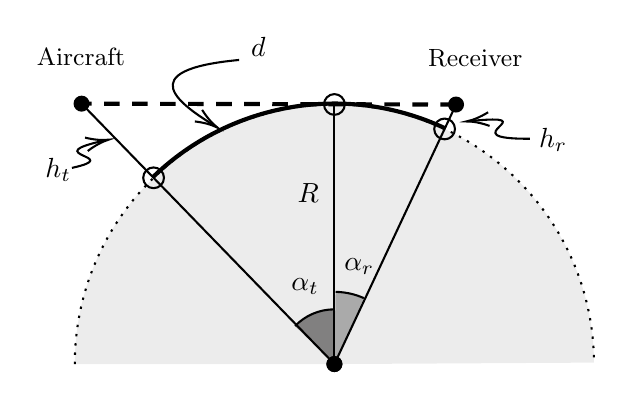
\begin{tikzpicture}[x=0.75pt,y=0.75pt,yscale=-1,xscale=1]
%uncomment if require: \path (0,447); %set diagram left start at 0, and has height of 447

%Shape: Arc [id:dp5690903281113118]
\draw  [draw opacity=0][fill={rgb, 255:red, 236; green, 236; blue, 236 }  ,fill opacity=1 ][dash pattern={on 0.84pt off 2.51pt}] (110.04,201) .. controls (110.04,201) and (110.04,201) .. (110.04,201) .. controls (110.04,131.93) and (166.04,75.93) .. (235.12,75.93) .. controls (303.96,75.93) and (359.82,131.55) .. (360.19,200.3) -- (235.12,201) -- cycle ; \draw  [dash pattern={on 0.84pt off 2.51pt}] (110.04,201) .. controls (110.04,201) and (110.04,201) .. (110.04,201) .. controls (110.04,131.93) and (166.04,75.93) .. (235.12,75.93) .. controls (303.96,75.93) and (359.82,131.55) .. (360.19,200.3) ;
%Straight Lines [id:da3652394426894523]
\draw [line width=1.5]  [dash pattern={on 5.63pt off 4.5pt}]  (293.72,75.96) -- (113.31,75.53) ;


%Curve Lines [id:da0314547922320223]
\draw    (329.24,92.44) .. controls (289.34,92.62) and (339.2,80.05) .. (300.48,83.92) ;
\draw [shift={(298.65,84.11)}, rotate = 353.97] [color={rgb, 255:red, 0; green, 0; blue, 0 }  ][line width=0.75]    (10.93,-3.29) .. controls (6.95,-1.4) and (3.31,-0.3) .. (0,0) .. controls (3.31,0.3) and (6.95,1.4) .. (10.93,3.29)   ;

%Curve Lines [id:da8824974860724117]
\draw    (108.67,106.48) .. controls (134.99,100.68) and (90.76,100.58) .. (124.73,93.23) ;
\draw [shift={(126.33,92.89)}, rotate = 528.24] [color={rgb, 255:red, 0; green, 0; blue, 0 }  ][line width=0.75]    (10.93,-3.29) .. controls (6.95,-1.4) and (3.31,-0.3) .. (0,0) .. controls (3.31,0.3) and (6.95,1.4) .. (10.93,3.29)   ;

%Shape: Arc [id:dp3560200749347655]
\draw  [draw opacity=0][line width=1.5]  (147.84,110.79) .. controls (184.2,75.63) and (239.86,64.64) .. (288.37,87.37) .. controls (288.48,87.42) and (288.58,87.47) .. (288.69,87.52) -- (235.12,201) -- cycle ; \draw  [line width=1.5]  (147.84,110.79) .. controls (184.2,75.63) and (239.86,64.64) .. (288.37,87.37) .. controls (288.48,87.42) and (288.58,87.47) .. (288.69,87.52) ;
%Curve Lines [id:da23413477884430978]
\draw    (189.2,54.48) .. controls (136.23,59.41) and (161.51,76.18) .. (177.22,86.1) ;
\draw [shift={(178.89,87.15)}, rotate = 212.24] [color={rgb, 255:red, 0; green, 0; blue, 0 }  ][line width=0.75]    (10.93,-3.29) .. controls (6.95,-1.4) and (3.31,-0.3) .. (0,0) .. controls (3.31,0.3) and (6.95,1.4) .. (10.93,3.29)   ;

%Shape: Arc [id:dp32891412685871013]
\draw  [draw opacity=0][fill={rgb, 255:red, 170; green, 170; blue, 170 }  ,fill opacity=1 ] (235.67,166.21) .. controls (240.53,166.29) and (245.15,167.36) .. (249.33,169.23) -- (235.12,201) -- cycle ; \draw   (235.67,166.21) .. controls (240.53,166.29) and (245.15,167.36) .. (249.33,169.23) ;
%Shape: Arc [id:dp7029066137990934]
\draw  [draw opacity=0][fill={rgb, 255:red, 129; green, 128; blue, 128 }  ,fill opacity=1 ] (216.18,182.64) .. controls (220.99,177.68) and (227.73,174.61) .. (235.17,174.63) -- (235.12,201) -- cycle ; \draw   (216.18,182.64) .. controls (220.99,177.68) and (227.73,174.61) .. (235.17,174.63) ;
%Straight Lines [id:da8761528166800212]
\draw    (293.72,75.96) -- (235.12,201) ;
\draw [shift={(235.12,201)}, rotate = 115.11] [color={rgb, 255:red, 0; green, 0; blue, 0 }  ][fill={rgb, 255:red, 0; green, 0; blue, 0 }  ][line width=0.75]      (0, 0) circle [x radius= 3.35, y radius= 3.35]   ;
\draw [shift={(293.72,75.96)}, rotate = 115.11] [color={rgb, 255:red, 0; green, 0; blue, 0 }  ][fill={rgb, 255:red, 0; green, 0; blue, 0 }  ][line width=0.75]      (0, 0) circle [x radius= 3.35, y radius= 3.35]   ;
%Straight Lines [id:da6955293230830237]
\draw    (235.12,75.53) -- (235.12,201) ;
\draw [shift={(235.12,201)}, rotate = 90] [color={rgb, 255:red, 0; green, 0; blue, 0 }  ][fill={rgb, 255:red, 0; green, 0; blue, 0 }  ][line width=0.75]      (0, 0) circle [x radius= 3.35, y radius= 3.35]   ;

%Straight Lines [id:da17629850181731288]
\draw    (235.12,201) -- (113.31,75.53) ;
\draw [shift={(113.31,75.53)}, rotate = 225.85] [color={rgb, 255:red, 0; green, 0; blue, 0 }  ][fill={rgb, 255:red, 0; green, 0; blue, 0 }  ][line width=0.75]      (0, 0) circle [x radius= 3.35, y radius= 3.35]   ;


% Text Node
\draw (102.11,107.26) node   [align=left] {$\displaystyle h_{t}$};
% Text Node
\draw (340.5,93.15) node   [align=left] {$\displaystyle h_{r}$};
% Text Node
\draw (222.56,118.43) node   [align=left] {$\displaystyle R$};
% Text Node
\draw (198.49,48) node   [align=left] {$\displaystyle d$};
% Text Node
\draw (113.05,53.17) node  [font=\small] [align=left] {Aircraft};
% Text Node
\draw (302.94,53.49) node  [font=\small] [align=left] {Receiver};
% Text Node
\draw (221,163.55) node   [align=left] {$\displaystyle \alpha _{t}$};
% Text Node
\draw (247.09,154.11) node   [align=left] {$\displaystyle \alpha _{r}$};

\draw   (288.21, 87.72) circle [x radius= 5, y radius= 5]   ;
\draw   (235.12, 75.93) circle [x radius= 5, y radius= 5]   ;
\draw   (148, 111.26) circle [x radius= 5, y radius= 5]   ;
\end{tikzpicture}

  \caption{Maximum receiver range}
  \label{fig:max_range}
\end{figure}


Knowing the altitude of the receiver antenna, it is possible to determine the maximum range ($d$) of a Mode~S receiver as:

\begin{align}
  d &= (\alpha_r + \alpha_t) R \\
  & = \left( \arccos \frac{R}{R+h_r} + \arccos \frac{R}{R+h_t} \right) R
\end{align}

\noindent where $R$ is the radius of the earth, while $h_t$ and $h_r$ are the height of the aircraft and receiver above the sea level. Using this equation, we can calculate the maximum receiving range for aircraft flying at different altitudes. In Figure \ref{fig:max_range_curve}, the maximum range curves calculated using several receiver heights are shown.

\begin{figure}[ht]
  \centering
  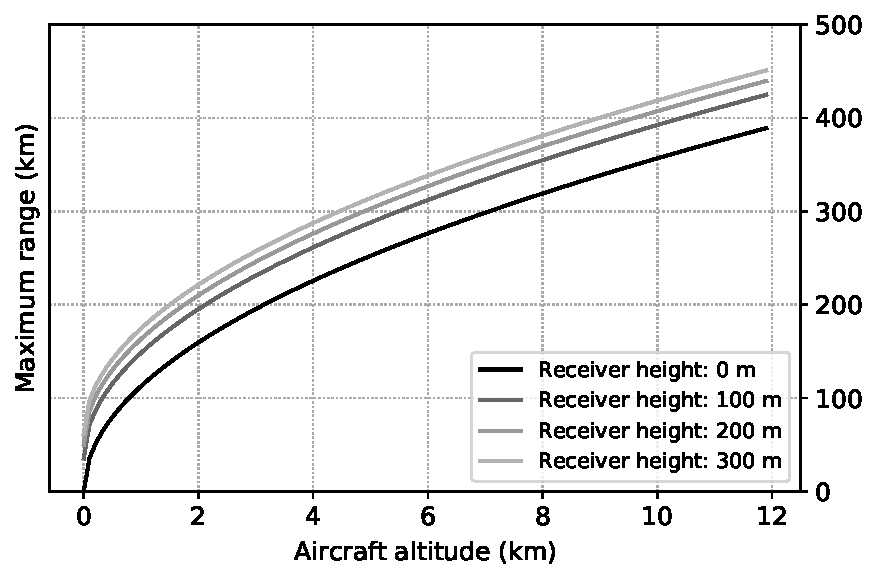
\includegraphics[scale=0.6]{figures/quickstart/max_range_curve.pdf}
  \caption{Maximum receiver range curve}
  \label{fig:max_range_curve}
\end{figure}


It should be noted that this figure shows the maximum radio range due to the curvature of the Earth. However, in real-life applications, Mode~S signal follows the Friis transmission model, which states that the maximum distance also depends on the power of the transmitter, as well as the directivities of the transmission and receiving antennas. When considering these factors, the actual radio range for the receiver might be more limited than the theoretical values shown in the previous figure.

\section{Antenna}
A large variety of commercial off-the-shelf antennas can be deployed to receive Mode~S signals. In principle, any antenna designed for the radio frequency around 1 GHz can be used for receiving Mode~S signals.

However, it is not difficult to design your own antenna. The carrier frequency of Mode~S is 1090 MHz, which corresponds to the wavelength of 27.5 centimeters. In order to have an antenna that is tuned to this specific frequency, one can design the antenna simply using a piece of a conductor (metal wire) and a coaxial feeder cable. In Figure \ref{fig:antennas}, a few common antenna designs are shown.

\begin{figure}[ht]
  \centering
  

\tikzset{every picture/.style={line width=0.75pt}} %set default line width to 0.75pt        

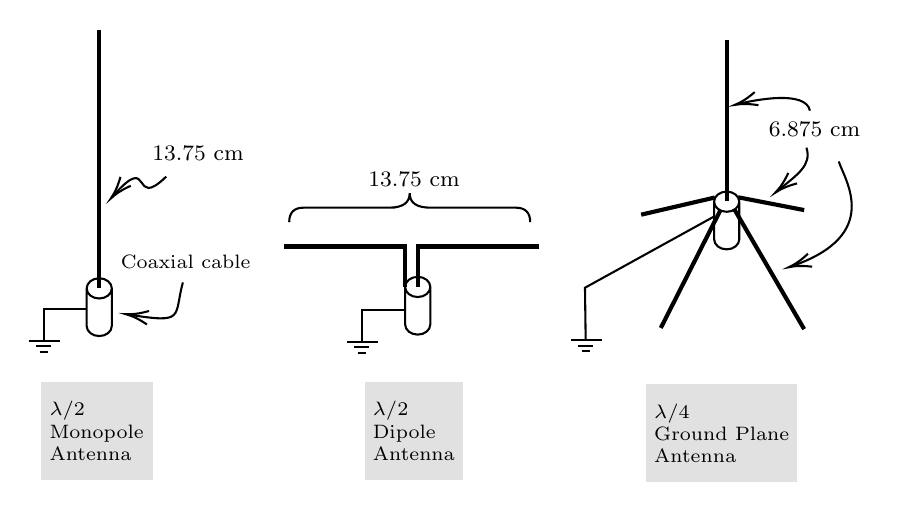
\begin{tikzpicture}[x=0.75pt,y=0.75pt,yscale=-1,xscale=1]
%uncomment if require: \path (0,285); %set diagram left start at 0, and has height of 285

%Flowchart: Magnetic Disk [id:dp9203753850829601] 
\draw   (73.36,147.61) -- (73.36,165.71) .. controls (73.36,168.4) and (70.65,170.58) .. (67.3,170.58) .. controls (63.96,170.58) and (61.25,168.4) .. (61.25,165.71) -- (61.25,147.61)(73.36,147.61) .. controls (73.36,150.3) and (70.65,152.48) .. (67.3,152.48) .. controls (63.96,152.48) and (61.25,150.3) .. (61.25,147.61) .. controls (61.25,144.92) and (63.96,142.73) .. (67.3,142.73) .. controls (70.65,142.73) and (73.36,144.92) .. (73.36,147.61) -- cycle ;
%Straight Lines [id:da34747813628770396] 
\draw [line width=1.5]    (67.3,23) -- (67.3,147.19) ;
%Flowchart: Magnetic Disk [id:dp8472157603764505] 
\draw   (375.67,105.84) -- (375.67,123.94) .. controls (375.67,126.63) and (372.96,128.81) .. (369.61,128.81) .. controls (366.27,128.81) and (363.56,126.63) .. (363.56,123.94) -- (363.56,105.84)(375.67,105.84) .. controls (375.67,108.53) and (372.96,110.71) .. (369.61,110.71) .. controls (366.27,110.71) and (363.56,108.53) .. (363.56,105.84) .. controls (363.56,103.15) and (366.27,100.97) .. (369.61,100.97) .. controls (372.96,100.97) and (375.67,103.15) .. (375.67,105.84) -- cycle ;
%Straight Lines [id:da5662262777033016] 
\draw [line width=1.5]    (369.61,28.01) -- (369.61,105.42) ;
%Straight Lines [id:da13460916170815418] 
\draw [line width=1.5]    (363.9,103.83) -- (328.4,112.1) ;
%Straight Lines [id:da574222375987339] 
\draw [line width=1.5]    (406.93,167.24) -- (373.44,109.74) ;
%Straight Lines [id:da3064624130741478] 
\draw [line width=1.5]    (337.87,166.68) -- (366.5,110.1) ;
%Straight Lines [id:da5811958206568459] 
\draw [line width=1.5]    (406.93,109.88) -- (375.11,103.72) ;
%Curve Lines [id:da621153715774825] 
\draw    (409.71,61.98) .. controls (407.71,51.96) and (383.15,56.82) .. (375.41,58.71) ;
\draw [shift={(373.51,59.2)}, rotate = 344.05] [color={rgb, 255:red, 0; green, 0; blue, 0 }  ][line width=0.75]    (10.93,-3.29) .. controls (6.95,-1.4) and (3.31,-0.3) .. (0,0) .. controls (3.31,0.3) and (6.95,1.4) .. (10.93,3.29)   ;
%Curve Lines [id:da20820331798614888] 
\draw    (408.04,79.8) .. controls (410.69,88.27) and (403.78,92.71) .. (394.49,100.3) ;
\draw [shift={(393,101.52)}, rotate = 320.19] [color={rgb, 255:red, 0; green, 0; blue, 0 }  ][line width=0.75]    (10.93,-3.29) .. controls (6.95,-1.4) and (3.31,-0.3) .. (0,0) .. controls (3.31,0.3) and (6.95,1.4) .. (10.93,3.29)   ;
%Curve Lines [id:da7479713733277822] 
\draw    (99.6,93.73) .. controls (82.14,110.65) and (93.56,81.03) .. (74.1,102.9) ;
\draw [shift={(72.87,104.31)}, rotate = 310.82] [color={rgb, 255:red, 0; green, 0; blue, 0 }  ][line width=0.75]    (10.93,-3.29) .. controls (6.95,-1.4) and (3.31,-0.3) .. (0,0) .. controls (3.31,0.3) and (6.95,1.4) .. (10.93,3.29)   ;
%Straight Lines [id:da9730091494366713] 
\draw    (33.33,172.81) -- (48.37,172.81) ;
%Straight Lines [id:da05895285604419476] 
\draw    (36.9,175.59) -- (44.14,175.59) ;
%Straight Lines [id:da324980097446699] 
\draw    (38.57,178.15) -- (42.47,178.15) ;

%Straight Lines [id:da3818709999372871] 
\draw    (40.57,172.7) -- (40.57,157.66) -- (61.29,157.66) ;
%Straight Lines [id:da4499961816622231] 
\draw    (294.52,172.39) -- (309.55,172.39) ;
%Straight Lines [id:da6922155263599932] 
\draw    (298.08,175.17) -- (305.32,175.17) ;
%Straight Lines [id:da4456696138094858] 
\draw    (299.75,177.74) -- (303.65,177.74) ;

%Straight Lines [id:da16679558461507527] 
\draw    (301.67,172.32) -- (301.34,147.3) -- (363.49,113.01) ;
%Straight Lines [id:da7355318584367416] 
\draw [line width=1.5]    (279.28,127.42) -- (220.81,127.42) -- (220.81,146.91) ;
%Straight Lines [id:da25011934904681166] 
\draw [line width=1.5]    (156.23,127.42) -- (214.7,127.42) -- (214.7,146.91) ;
%Flowchart: Magnetic Disk [id:dp2241547095005254] 
\draw   (226.81,146.91) -- (226.81,165.01) .. controls (226.81,167.7) and (224.1,169.88) .. (220.75,169.88) .. controls (217.41,169.88) and (214.7,167.7) .. (214.7,165.01) -- (214.7,146.91)(226.81,146.91) .. controls (226.81,149.6) and (224.1,151.78) .. (220.75,151.78) .. controls (217.41,151.78) and (214.7,149.6) .. (214.7,146.91) .. controls (214.7,144.22) and (217.41,142.04) .. (220.75,142.04) .. controls (224.1,142.04) and (226.81,144.22) .. (226.81,146.91) -- cycle ;
%Straight Lines [id:da19895333176103813] 
\draw    (186.57,173.22) -- (201.61,173.22) ;
%Straight Lines [id:da8931773949500925] 
\draw    (190.14,176.01) -- (197.38,176.01) ;
%Straight Lines [id:da22035216453021045] 
\draw    (191.81,178.57) -- (195.71,178.57) ;

%Straight Lines [id:da35718244675007793] 
\draw    (193.81,173.11) -- (193.81,158.08) -- (214.53,158.08) ;
%Shape: Brace [id:dp32284987028621814] 
\draw   (274.94,115.72) .. controls (274.94,111.05) and (272.61,108.72) .. (267.94,108.72) -- (226.88,108.72) .. controls (220.21,108.72) and (216.88,106.39) .. (216.88,101.72) .. controls (216.88,106.39) and (213.55,108.72) .. (206.88,108.72)(209.88,108.72) -- (165.83,108.72) .. controls (161.16,108.72) and (158.83,111.05) .. (158.83,115.72) ;
%Curve Lines [id:da030068990122400274] 
\draw    (423.63,86.49) .. controls (426.39,95.31) and (444.98,121.87) .. (400.77,136.99) ;
\draw [shift={(399.41,137.44)}, rotate = 341.88] [color={rgb, 255:red, 0; green, 0; blue, 0 }  ][line width=0.75]    (10.93,-3.29) .. controls (6.95,-1.4) and (3.31,-0.3) .. (0,0) .. controls (3.31,0.3) and (6.95,1.4) .. (10.93,3.29)   ;
%Curve Lines [id:da013796374008901102] 
\draw    (107.6,144.73) .. controls (103.09,161.65) and (108.89,164.58) .. (81.71,160.27) ;
\draw [shift={(80,160)}, rotate = 369.15] [color={rgb, 255:red, 0; green, 0; blue, 0 }  ][line width=0.75]    (10.93,-3.29) .. controls (6.95,-1.4) and (3.31,-0.3) .. (0,0) .. controls (3.31,0.3) and (6.95,1.4) .. (10.93,3.29)   ;

% Text Node
\draw (114.92,82.59) node  [font=\footnotesize] [align=left] {13.75 cm};
% Text Node
\draw (411.94,70.89) node  [font=\footnotesize] [align=left] {6.875 cm};
% Text Node
\draw  [draw opacity=0][fill={rgb, 255:red, 225; green, 225; blue, 225 }  ,fill opacity=1 ]  (39.04,192.73) -- (93.04,192.73) -- (93.04,239.73) -- (39.04,239.73) -- cycle  ;
\draw (66.04,216.23) node  [font=\scriptsize] [align=left] {$\displaystyle \lambda /2\ $\\Monopole\\Antenna};
% Text Node
\draw  [draw opacity=0][fill={rgb, 255:red, 225; green, 225; blue, 225 }  ,fill opacity=1 ]  (330.72,193.73) -- (403.72,193.73) -- (403.72,240.73) -- (330.72,240.73) -- cycle  ;
\draw (367.22,217.23) node  [font=\scriptsize] [align=left] {$\displaystyle \lambda /4\ $\\Ground Plane\\Antenna};
% Text Node
\draw (218.97,95.12) node  [font=\footnotesize] [align=left] {13.75 cm};
% Text Node
\draw  [draw opacity=0][fill={rgb, 255:red, 225; green, 225; blue, 225 }  ,fill opacity=1 ]  (195.36,192.73) -- (242.36,192.73) -- (242.36,239.73) -- (195.36,239.73) -- cycle  ;
\draw (218.86,216.23) node  [font=\scriptsize] [align=left] {$\displaystyle \lambda /2\ $\\Dipole\\Antenna};
% Text Node
\draw (108.92,134.59) node  [font=\scriptsize] [align=left] {Coaxial cable};


\end{tikzpicture}

  \caption{Common antenna designs}
  \label{fig:antennas}
\end{figure}

The monopole antenna and the dipole antenna both are half-wavelength ($\lambda/2$) antennas with a total conductor length of 13.75 cm. The ground plan antenna is a quarter-wavelength ($\lambda/4$) antenna, where the main pole is 6.875 cm.

For a remote installation where the antenna is far from the receiver (i.e. long coaxial cable between the antenna and receiver), the high-frequency signal of Mode~S can attenuate quickly. When the signal has arrived at the receiver end, the signal to noise ratio can become quite high. To overcome this limitation, an active antenna may be used.

The active antenna has a low-noise amplifier integrated at the antenna side. Sometimes, it also includes a band-pass filter that is designed for 1090 MHz. The active antenna requires additional powering. Power is commonly supplied through a bias-tee device (Figure \ref{fig:biastee}) connected at the receiver end, which is on the left-hand side of the diagram. On the right-hand side, the radio frequency is mixed with the DC component, which allows the electronic circuit to be powered close to the receiver end.

\begin{figure}[ht]
  \centering
  

\tikzset{every picture/.style={line width=0.75pt}} %set default line width to 0.75pt

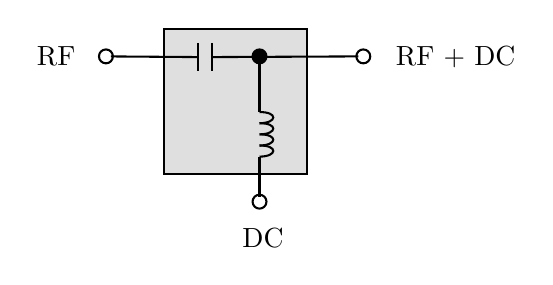
\begin{tikzpicture}[x=0.75pt,y=0.75pt,yscale=-1,xscale=1]
%uncomment if require: \path (0,300); %set diagram left start at 0, and has height of 300

%Shape: Rectangle [id:dp5847419531167373]
\draw  [fill={rgb, 255:red, 223; green, 223; blue, 223 }  ,fill opacity=1 ] (94,26.67) -- (162.67,26.67) -- (162.67,96.67) -- (94,96.67) -- cycle ;
%Straight Lines [id:da3655997692264292]
\draw    (68.35,40.02) -- (110.5,40.34) ;
\draw [shift={(66,40)}, rotate = 0.44] [color={rgb, 255:red, 0; green, 0; blue, 0 }  ][line width=0.75]      (0, 0) circle [x radius= 3.35, y radius= 3.35]   ;
%Straight Lines [id:da4762508902899607]
\draw    (117.13,40.34) -- (187.65,40.01) ;
\draw [shift={(190,40)}, rotate = 359.73] [color={rgb, 255:red, 0; green, 0; blue, 0 }  ][line width=0.75]      (0, 0) circle [x radius= 3.35, y radius= 3.35]   ;
%Straight Lines [id:da03465082932527963]
\draw    (110.5,33.51) -- (110.5,47.17) ;
%Straight Lines [id:da3348158883114294]
\draw    (117.13,33.51) -- (117.13,47.17) ;
%Straight Lines [id:da9848210218655242]
\draw    (140,40) -- (140,66.84) ;
\draw [shift={(140,40)}, rotate = 90] [color={rgb, 255:red, 0; green, 0; blue, 0 }  ][fill={rgb, 255:red, 0; green, 0; blue, 0 }  ][line width=0.75]      (0, 0) circle [x radius= 3.35, y radius= 3.35]   ;
%Straight Lines [id:da6955712196773951]
\draw    (140,88.31) -- (140,107.65) ;
\draw [shift={(140,110)}, rotate = 90] [color={rgb, 255:red, 0; green, 0; blue, 0 }  ][line width=0.75]      (0, 0) circle [x radius= 3.35, y radius= 3.35]   ;
%Curve Lines [id:da44310646563351463]
\draw    (140,66.84) .. controls (148.95,66.73) and (148.72,72.1) .. (140,72.21) ;
%Curve Lines [id:da7249179830921086]
\draw    (140,72.21) .. controls (148.95,72.1) and (148.72,77.47) .. (140,77.58) ;
%Curve Lines [id:da23791689791160175]
\draw    (140,77.58) .. controls (148.95,77.47) and (148.72,82.84) .. (140,82.95) ;
%Curve Lines [id:da12134770027518282]
\draw    (140,82.95) .. controls (148.95,82.84) and (148.72,88.21) .. (140,88.31) ;

% Text Node
\draw (42,39.83) node   [align=left] {RF};
% Text Node
\draw (234.5,40.5) node   [align=left] {RF + DC};
% Text Node
\draw (141.66,127.5) node   [align=left] {DC};


\end{tikzpicture}

  \caption{Bias-tee diagram}
  \label{fig:biastee}
\end{figure}


\section{Receiver}

Many modern Mode~S receivers are built using software-defined radio (SDR). An SDR usually can be tuned to a wide range of radio frequencies. The user can conveniently select the center frequency of the receiver and the sampling rate, as well as defined the bandwidth of the onboard low-pass filter if it is supported.

For receiving ADS-B (and other types of Mode~S message), a RTL-SDR is the most common type of low-cost receiver to choose. Many different brands of RTL-SDR receivers exist; they are often built with the Realtek RTL2832U chipset. It can work with radio frequencies from 24 to 1766 MHz. The maximum sampling rate is 2.8 million samples per second (MSPS). Given that a Mode~S bit consists of a pulse cycle of 2 microseconds (see Figure \ref{fig:mode_s_uplink_pulses}), the minimum SDR sampling rate required for Mode~S is 2 MSPS. RLT-SDR devices just barely manage to meet this requirement.

\begin{notebox}{Note}
  The maximum frequency range of RTL-SDR can be from 0 to 2220 MHz. However, the sensitivity drops off significantly outside the 24 - 1766 MHz range. The sampling rate can actually go up to a maximum of 3.2 million samples per second, but some samples may be dropped at this sampling rate. Hence, it is not stable.
\end{notebox}

SDRs that offer a higher performance also exist. They often support a larger frequency range with higher sampling rates. Some offer multiple transmiting (TX) and receiving (RX) channels. In Table \ref{tb:sdr}, a few examples of common SDR devices are given. The performance of RTL-SDR is listed as a comparison.

\begin{table}[ht]
  \footnotesize
  \caption{Examples of common software defined radio devices}
  \label{tb:sdr}
  \begin{tabular}{|l|l|l|l|l|l|}
  \hline
   & \textbf{RTL-SDR} & \textbf{AirSpy R2} & \textbf{HackRF 1} & \textbf{LimeSDR} & \textbf{BladeRF 2} \\ \hline
  \textbf{Frequency (from)} & 24 MHz & 24 MHz & 1 MHz & 100 KHz & 47 MHz \\ \hline
  \textbf{Frequency (to)} & 1766 MHz & 1700 MHz & 6000 MHz & 3800 MHz & 6000 MHz \\ \hline
  \textbf{Max sample rate} & 2.8 MSPS & 10 MSPS & 20 MSPS & 61.44 MSPS & 61.44 MSPS \\ \hline
  \textbf{RX channels} & 1 & 1 & 1 & 2 & 2 \\ \hline
  \textbf{TX channels} & 0 & 1 & 1 & 2 & 2 \\ \hline
  \textbf{Open hardware} & No & Firmware & Full & Full & \begin{tabular}[c]{@{}l@{}}Firmware,\\ Schematics\end{tabular} \\ \hline
  \end{tabular}
\end{table}

\section{Software tools}

Several software tools are also available to work with some of these SDR devices and decode Mode~S and ADS-B signals directly. In this section, we explain how to use two open-source tools, which are \texttt{dump1090} and \texttt{pyModeS}.

\subsection{dump1090}

\texttt{dump1090} is the most well-known open-source Mode~S decoder currently available. The software is written in C programming language and was originally developed by Salvatore Sanfilippo \footnote{https://github.com/antirez/dump1090} under the BSD three clause license.

Since its release in 2013, the repository has been forked and extended intensively on GitHub, creating more than 900 forks so far. Many of the branched versions contain different variations, such as support for additional hardware, additional decoded Mode~S messages, and additional output format. Currently, one of the most comprehensive forks is the repository maintained by FlightAware.\footnote{https://github.com/flightaware/dump1090} The following examples will be based on the FlightAware version of \texttt{dump1090}, using a Debian based Linux system.

\subsubsection{Installation of dump1090}
The latest version of \texttt{dump1090} source code can download as follows:

\begin{verbatim}
$ git checkout https://github.com/flightaware/dump1090.git
\end{verbatim}

Before compiling the code, following dependencies must be installed:

\begin{verbatim}
sudo apt-get install build-essential debhelper librtlsdr-dev \
  pkg-config dh-systemd libncurses5-dev libbladerf-dev
\end{verbatim}

Next, we can compile the source code as:

\begin{verbatim}
$ cd dump1090
$ make
\end{verbatim}

It is worth noting that the FlightAware version of \texttt{dump1090} supports both RTL-SDR and BladeRF devices by default.

\subsubsection{Default usage of dump1090}

Once it is compiled and the RTL-SDR receiver is connected, we can run the following command to start receiving and decoding signals:

\begin{verbatim}
$ ./dump1090
\end{verbatim}

With the default option, Mode~S messages and decoded information are displayed in the terminal. For example:

\begin{verbatim}
*8d451dbd9905b5018004005979c5;
CRC: 000000
RSSI: -20.6 dBFS
Score: 1800
Time: 9214131.08us
DF:17 AA:451DBD CA:5 ME:9905B501800400
 Extended Squitter Airborne velocity over ground, subsonic (19/1)
  ICAO Address:  451DBD (Mode~S / ADS-B)
  Air/Ground:    airborne
  Ground track   271.4
  Groundspeed:   436.1 kt
  Geom rate:     0 ft/min
  NACv:          0
\end{verbatim}

\subsubsection{Raw Mode~S messages}

If we only want to display the  raw messages, the \texttt{--raw} option can be provided, as follows:

\begin{verbatim}
$ ./dump1090 --raw
\end{verbatim}

In this case, the terminal output will only contain the raw messages:

\begin{verbatim}
*5d4074358ad00c;
*8d407435990dbd01900484f66c3c;
*8d40743558af828cd326fe0c2fe9;
*a00015b8c2680030a80000318667;
*a80011b1e0da112fe0140060939f;
*a00015b8c2680030a80000318667;
*5d4074358ad030;
*5d4074358ad030;
\end{verbatim}

\subsubsection{Interactive mode}

\texttt{dump1090} can also provide a live view of all aircraft seen by the receiver through the use of the \texttt{--interactive} option:

\begin{verbatim}
$ ./dump1090 --interactive
\end{verbatim}

An example of the terminal output is shown in Figure \ref{fig:dump1090}.

\begin{figure}[ht]
  \centering
  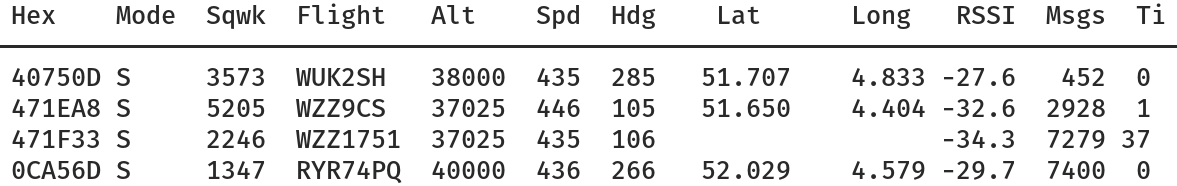
\includegraphics[scale=0.33]{figures/quickstart/dump1090.png}
  \caption{Example of a dump1090 interactive output}
  \label{fig:dump1090}
\end{figure}


% An example of the terminal output for the interactive view is shown as follows:

% \begin{verbatim}
% Hex    Mode~Sqwk Flight  Alt    Spd  Hdg   Lat    Long   RSSI   Msgs  Ti
% ------------------------------------------------------------------------
% 40750D S    3572 WUK2SH  38000  435  285  51.707  4.833  -27.6   452   0
% 471EA8 S    5205 WZZ9CS  37025  446  105  51.650  4.404  -32.6  2928   1
% 471F33 S    2246 WZZ1751 37025  435  106                 -34.3  7279  37
% 0CA56D S    1347 RYR74PQ 40000  436  266  52.029  4.579  -29.7  7400   0
% \end{verbatim}
  


\subsection{pyModeS}
\texttt{pyModeS} is an open-source Mode~S decoder project that I started in 2015, during my PhD research at TU Delft. It is a library that was originally designed to focus on lower level inference and decoding of individual raw Mode~S messages. Many users of \texttt{pyModeS} were researchers or developers who needed a Mode~S decoder package in the Python programming language. Later on, hardware support and live decoding were added, which made it more akin to \texttt{dump1090} of late.


\subsubsection{Installation of pyModeS}

As a Python library, it is possible to install the most recent stable version of \texttt{pyModeS} as:

\begin{verbatim}
pip install pyModeS
\end{verbatim}

The latest development version for the GitHub can be installed as:

\begin{verbatim}
pip install git+https://github.com/junzis/pyModeS
\end{verbatim}


\subsubsection{Live traffic view}

\texttt{pyModeS} provides the possibility to view live traffic through the \texttt{modeslive} command. The usage of this command is shown as follows:

\begin{verbatim}
$ modeslive [-h] --source SOURCE [--connect SERVER PORT DATAYPE]
            [--latlon LAT LON] [--show-uncertainty] [--dumpto DUMPTO]

arguments:
 -h, --help            show this help message and exit
 --source SOURCE       Choose data source, "rtlsdr" or "net"
 --connect SERVER PORT DATATYPE
                       Define server, port and data type. Supported data
                       types are: ['raw', 'beast', 'skysense']
 --latlon LAT LON      Receiver latitude and longitude, needed for the surface
                       position, default none
 --show-uncertainty    Display uncertainty values, default off
 --dumpto DUMPTO       Folder to dump decoded output, default none
\end{verbatim}

When an RTL-SDR device is connected, the following command can be used to display live traffic:

\begin{verbatim}
$ modeslive --source rtlsdr
\end{verbatim}

Data source can also be supplied through the network (for example, from \texttt{dump1090} TCP output stream) as:



\begin{verbatim}
$ dump1090 --net --quiet
$ modeslive --source net --connect localhost 30002 raw
\end{verbatim}

An example of the live view is shown in Figure \ref{fig:modeslive}.

\begin{figure}[ht]
  \centering
  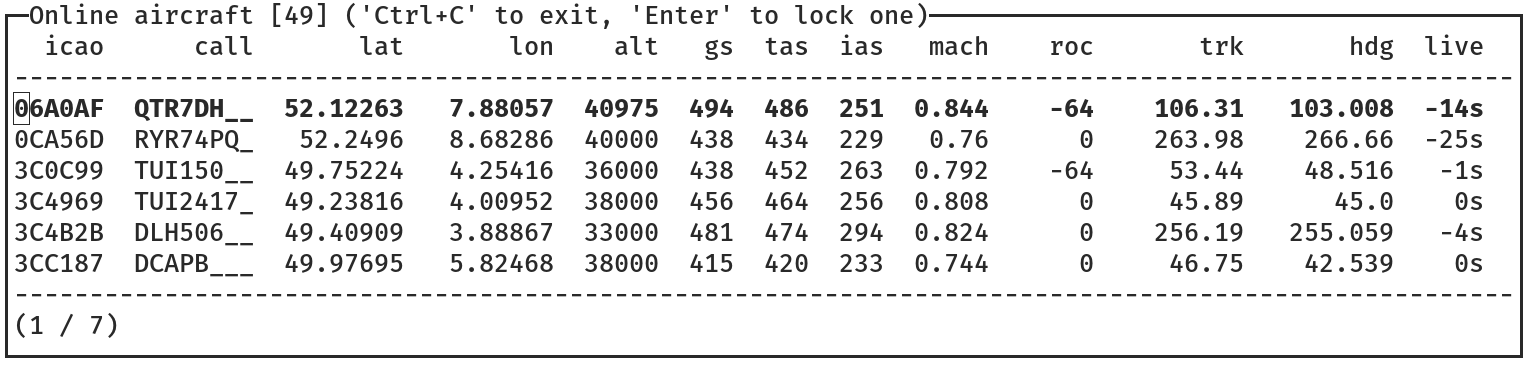
\includegraphics[scale=0.3]{figures/quickstart/modeslive.png}
  \caption{Example of a \texttt{modeslive} aircraft live view}
  \label{fig:modeslive}
\end{figure}


\subsubsection{Programming interface}

Since \texttt{pyModeS} is designed as a low-level development library, its decoding functionalities can be easily accessed in Python. Some examples of accessing \texttt{pyModeS} are shown here.

Core functions that provide access to extract the Downlink Format, ICAO address, ADS-B Type Code, as well as to perform parity check. For example:

\begin{verbatim}
import pyModeS as pms

pms.df(msg)         # Downlink Format
pms.icao(msg)       # Infer the ICAO address from the message
pms.crc(msg)        # Perform parity check
pms.typecode(msg)   # Obtain ADS-B message Type Code
\end{verbatim}


ADS-B related functions allow information such as identity, position, and velocities to be decoded. For example:

\begin{verbatim}
# position messages
pms.adsb.position(msg_even, msg_odd, t_even, t_odd)
pms.adsb.altitude(msg)

# velocity messages
pms.adsb.velocity(msg)
\end{verbatim}

There are also a large number of functions designed to infer and decode Mode~S downlink messages. For example:

\begin{verbatim}
# Mode~S DF=4/20 altitude code
pms.common.altcode(msg)

# Mode~S DF=5/21 squwak code
pms.common.idcode(msg)

# Infer the Modes-S BDS code
pms.bds.infer(msg)

# BDS 4,0
pms.commb.selalt40mcp(msg)  # MCP/FCU selected altitude (ft)
pms.commb.selalt40fms(msg)  # FMS selected altitude (ft)
pms.commb.p40baro(msg)      # Barometric pressure (mb)

# BDS 5,0
pms.commb.roll50(msg)       # Roll angle (deg)
pms.commb.trk50(msg)        # True track angle (deg)
pms.commb.gs50(msg)         # Ground speed (kt)
pms.commb.rtrk50(msg)       # Track angle rate (deg/sec)
pms.commb.tas50(msg)        # True airspeed (kt)

# BDS 6,0
pms.commb.hdg60(msg)        # Magnetic heading (deg)
pms.commb.ias60(msg)        # Indicated airspeed (kt)
pms.commb.mach60(msg)       # Mach number (-)
pms.commb.vr60baro(msg)     # Barometric altitude rate (ft/min)
pms.commb.vr60ins(msg)      # Inertial vertical speed (ft/min)
\end{verbatim}

There are several commonly used functions related to Mode~S decoding. A complete list of the APIs can be found in the \texttt{pyModeS} library API documentation.

In the rest of this book, most of the decoding details with be explained, which will often reflect the source code from \texttt{pyModeS}.
